\section{Related Work} \label{sec:related-work}

We briefly provide an overview of existing research on \CGSs{} to explain why
it doesn't addressed problems we intend to address in this proposal.
There exists a large body of research on \CGSs{}. In
\cite{PelegJBI13}, the author provides a methodological review of
existing work on Computer Interpretable Guidelines (\CIGs{}): executable
formalizations of \BPGs{} used to construct \CGSs{}.
Existing work is classified into one of eight themes spanning
the entire development cycle of a \CIG{}. The themes and relations between them
are shown in \figurename{} \ref{fig:cpg-research-topics}.

\begin{wrapfigure}{l}{0.5\textwidth}
  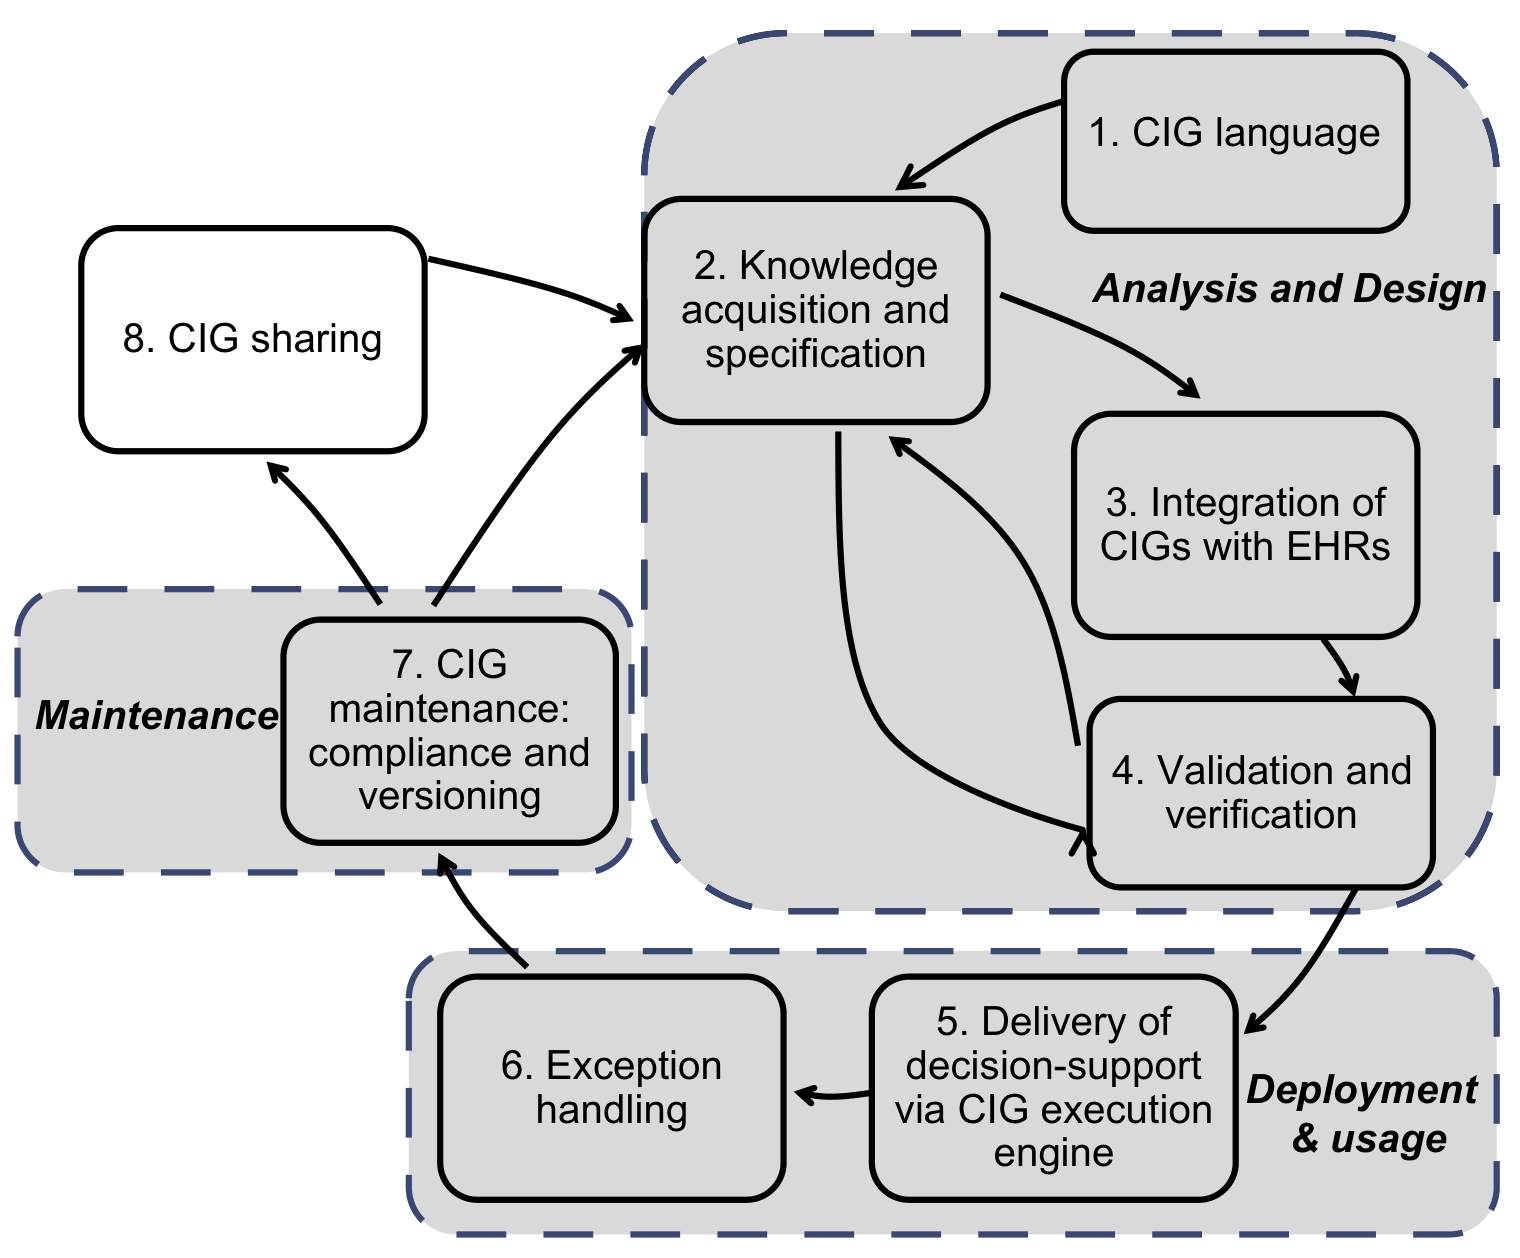
\includegraphics[width=\linewidth]{cpg-topics}
  \caption{\CGSs{} Research Themes}\label{fig:cpg-research-topics}
\end{wrapfigure}

According to the author in \cite{PelegJBI13}, \CIGs{} are usually based on previously published non-executable
\BPGs{}. To develop a \CIG{}, a language is identified in (1). Teams of
software developers and clinicians then collaborate to express medical knowledge
in the \BPG{} in the identified language. In (3), the \CIG{}
is integrated with components such as a Graphical User
Interface (\GUI{}), Electronic Health Records (\EHRs{}) and external devices
(such as monitors for patient parameters) to obtain a \CGS. Before adoption
in the real-world, it is imperative to ensure that the \CIG{} \emph{mirrors}
the underlying \BPG{}. This validation occurs by \emph{testing} the \CGS{}
using execution capabilities of the modeling language from (1) in (5).
Additionally, formal verification may be used to establish other desired
properties hold. Inconsistencies identified in (5) are fixed through developer-clinician
collobaration in (2),  re-validation and
verification. While the aforementioned development cycle has resulted in several
effective \CGSs{}, it has some limitations:

\paragraph{Gap between specification and implementation:}

To develop the \CIG{}, software developers rely on clinicians to interpret the
non-executable \BPG{} and communicate
the intended semantics to them. Thus, the non-executable \BPG{} serves as a functional specification for
the \CIG{}, i.e. the implementation. In such safety-critical systems, it is
imperative that the implementation, i.e. the \CIG{}, conforms to its
specification, i.e., the \BPG{}. To address this, the \CIG{} is tested by
putting the \CGS{} through clinical simulations. But, while testing reduces
the risk of non-conformance, it does not completely eliminate it.

\paragraph{Safe Modularity:}

While developing \CGSs{} is both complex and cost-intensive,
the development effort can be reduced by sharing \CGSs{} across hospitals \cite{PelegAMIA00}.
But, even for the same \BPG{}, hospitals develop their own \CGSs{} to address
their needs, resulting in duplicated work.
For instance, for the \ACLS{} \BPG{}, multiple \CGSs{} have been developed by different
different hospitals in a span of just six years years \cite{FullCodePro,PediAppRREST2020,
PediAppRREST2021,GuidingPad2017,GuidingPad2019, GuidingPad2020,DST2014,DST2019,ROSCo2021,TeamScreen2019,Wu2017}.
\CGSs{} based on the same \BPG{} typically have the same \CIG{}, but may differ
in their Graphical User Interfaces (\GUIs), or integration with external
devices, to address hospital-specific needs.
To enable safe sharing of knowledge, we need a mechanism that:
\begin{enumerate*}[label=(\alph*)]
  \item allows a stable, formally-verfied \CIG{} that is \emph{decoupled} from other
    components, and,
  \item supports hospital-specific customizations without compromising system
    \emph{safety}.
\end{enumerate*}

\paragraph{Holistic System Safety:}

Actions performed by a \CGS{} can either be \emph{programming-oriented}
or \emph{clinically-oriented} \cite{BoxwalaJBI04}. \emph{programming-oriented}
actions are peformed by executing the \CIG{} itself. For example,
using patient parameters, or health records to make a reccomendation or diagnosis,
or to raise a warning. \emph{clinically-oriented} actions on the other hand
are ones that involve a clinician. For example, in the case of \ACLS{},
the \CGS{} recommends that Cardiopulmonary Resuscitation (\CPR{}) be performed
for a certain length of time. Such actions can only be performed by clinicians,
an the \CGS{} assumes that the recommended action was indeed performed before
moving resuming guidance.

For holistic system safety, both categories of actions must be completed
successfully. While traditional formal reasoning techniques can be employed
to establish correctness of \emph{programming-oriented} actions, the same
cannot be used to reason about \emph{clinically-oriented} ones.
Thus, a mechanism that allows some guarantees about clinically-oriented is
desirable.


\paragraph{Formal Semantics:}

Since \CIGs{} are safety-critical, it is vital that the
language in which they're developed has complete formal semantics that
can be used to derive tools such as semantically-correct interpreters,
deductive program verifiers, and model-checkers.

\subsection{Limitations of Existing Approaches}

While existing approaches have been imperative to increasing \CGS{} adoption, to the
best of our knowledge, none of them address all of the aforementioned
limitations. We briefly describe notable approaches, their successes, and their limitations.

The Arden Syntax \cite{HripcsakCBM94} a widely used medium for
expressing \CIGs{}.  Guidelines as described using Medical
Logic Modules that contains information related to guideline's purpose
, maintainance, and medical knowledge. The modules are modular to allow
re-use and sharing across hospitals. But, Arden Syntax
is focused on describing simple, modular, and independent
guidelines (such as reminders), and not on guidelines with complex logic (such
as treatment protocols) \cite{PelegJBI01}.
Arden Syntax's limitation in modeling complexity is addressed by
GLIF \cite{BoxwalaJBI04}: a language that uses flowcharts to expressed
guidelines. A multi-level approach is
employed to manage complexity: at the top is the conceptual level, where
only high-level details relevant for human-comprehension are present. In the
middle is a computable-level, where details of guideline execution flow
and patient data elements are specified. At the bottom is the implementable
level, where institution-specific details and mappings into patient data are
specified. Both Arden Syntax and GLIF  eliminate
the gap between the \BPG{}, i.e. the specification, and the \CIG{}, i.e. implementation as
they're meant to be either directly used by clinicians (or in collaboration with
computer scientists) to express \BPGs{} in an executable medium. \CIGs{}
expressed in them are meant to be shared across hospitals, and are thus modular.
However, neither formalism has complete formal semantics, or comprehensiev support for
rigorous formal analysis.

The need for formal analysis is identified by Asbru: a formalism with formally
defined syntax and semantics \cite{ShaharAMIA96}. In Asbru, a guideline is modeled as a plan
that contains:
\begin{enumerate*}[label=(\roman*)]
  \item intentions that define aims,
  \item conditions that specify when the plan is applicable,
  \item effects that define expected behavior during execution, and,
  \item a body containing other subplans.
\end{enumerate*}
Apart from an execution engine, the Asbru ecosystem also contains
other tools, such as a model checker for verification \cite{BaumlerSPIN06}.
However, the formal semantics of Asbru have been only partially defined, and
is insufficient to implement tools for the language \cite{SuttonAMIA03}.
The importance of a complete formal-semantics is identified and addressed
by PROforma \cite{SuttonAMIA03}, another formalism that uses plans to
model guidelines. A PROforma plan is made of a sequence of tasks.
The plan defines constraints on their enactment, and circumstances
for termination (for example, exceptions) \cite{SuttonAMIA03}. But, despite
having complete formal semantics, it does not have a comprehensive suite of
formal analysis tools such as model checkers, deductive verifiers.


The SAGE guideline model \cite{TuSAGE04} uses the Prot\'eg\'e knowledge
representation framework \cite{NoyAMIA03} to model guidelines,
and improves on aforementioned approaches by
enabling seamless integration into hospitals' existing Clinical Information Systems
(\CISs). But, it lacks complete formal semantics, and analysis tools
such as deductive verifiers and model checkers.
The GLARE formalism \cite{TerenzianiBook04} uses an actions based approach
to represent guidelines, and addresses clnician-comprehensibility and
modularity. For formal analysis, GLARE guidelines can be translated to
Promela: the SPIN model checker's specification language \cite{GiordanoAMIA06}.
The approach partly addresses holistic safety as
external agents (such as clinicians) can be modelled and analyzed.
But, the scenario where the external agent's behavior
deviates from the model during system execution isn't addressed.
Non medical-domain specific languages can also be used to reason about
medical systems. For example, in \cite{ArcainiMEMCODE15}, Abstract State
Machines (\ASMs) are used to validate and verify a system for measuring
patients' stereoacuity in the diagnosis of amyblyopia. But such a
formalism, while suitable for formal verification, may
not be easily comprehensible to clinicians for validation.

In \tablename{} \ref{table:existing-approaches}, we provide an overview of
the strengths and limitations of existing approaches. Note that we use
\greencheck{}, \cancelcheck{}, and \redcross{} to depict that an approach
fully-addresses, partly-addresses, or doesn't address a limitation respectively.
To the best of our knowledge,
none of the aforementioned approaches have:
\begin{itemize}[leftmargin=*]
  \setlength\itemsep{0em}
  \item An interpreter or execution engine with \emph{\underline{correctness guarantees}}.
  \item A Rich Suite of \emph{\underline{formal analysis tools}} such as a deductive program
    verifier, model checker, and symbolic execution engine that can be used to
    reason about the guidelines. Since a \CIG{} can comprise multiple
    processes that are \emph{parallel}, \emph{sequential}, or a mix of both,
    reasoning about them can be challenging. But, existing work in modeling
    and reasoning about distributed systems can provide solutions.
  \item Ability to reason about agents that perform \emph{\underline{external
    agents}}. These include clinicians responsible for \emph{clinically-defined}
    actions, or \emph{monitors} for \emph{patient parameters}. While it may seem
    impossible to reason about systems that depend heavily on actions of
    external agents, solutions to similar problems in other domains, such as
    the Simplex Architecture \cite{BakRTAS09} in Real-Time Systems (\RTSs), can be looked at for directions.
\end{itemize}

\begin{center}
\renewcommand{\arraystretch}{0.5}
%\setlength\extrarowheight{-9pt}
  \begin{table}
  \begin{tabularx}{\textwidth}{
      >{\centering\arraybackslash}X
    || >{\centering\arraybackslash}X
    | >{\centering\arraybackslash}X
    | >{\centering\arraybackslash}X
    | >{\centering\arraybackslash}X
  }
                 & Implementation-Specification Gap & Complete Formal Semantics & Formal Analysis Tools & Holistic Safety  \\
    Arden Syntax & $\greencheck$                               & $\redcross$               & $\redcross$           & $\redcross$ \\
    GLIF         & $\greencheck$                               & $\redcross$               & $\redcross$           & $\redcross$ \\
    Asbru        & $\greencheck$                               & $\cancelcheck$            & $\greencheck$         & $\redcross$ \\
    PROForma     & $\greencheck$                               & $\greencheck$             & $\redcross$           & $\redcross$ \\
    GLARE        & $\greencheck$                               & $\cancelcheck$            & $\cancelcheck$        & $\cancelcheck$ \\
    Promela/SPIN & $\redcross$                                 & $\greencheck$             & $\greencheck$         & $\cancelcheck$ \\
    AMSs         & $\redcross$                                 & $\greencheck$             & $\greencheck$         & $\redcross$ \\
    SAGE         & $\greencheck$                               & $\redcross$               & $\redcross$           & $\redcross$ \\
  \end{tabularx}
  \caption{Comparison of Existing Approaches}\label{table:existing-approaches}
  \end{table}
\end{center}
